\chapter{Methods}
%(5-7 pages)

\section{Design}
%-------------------------------------------%

\begin{figure}[h]
	\centering
    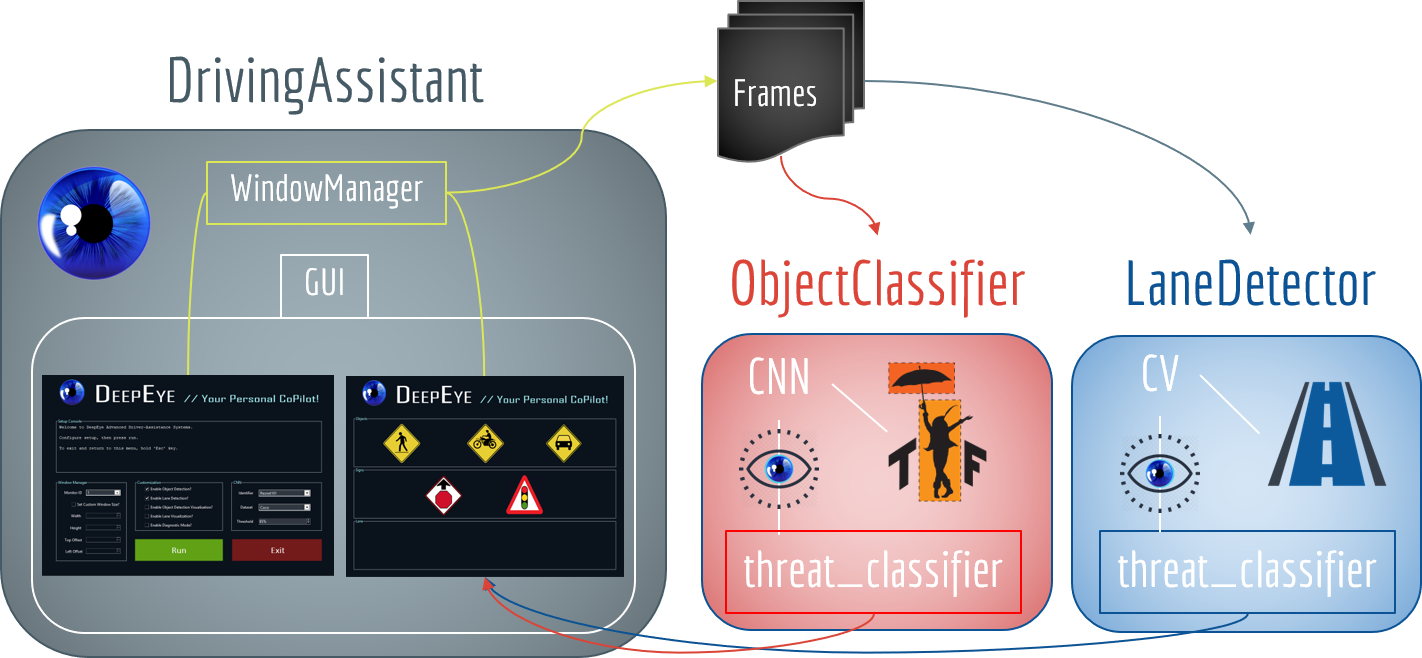
\includegraphics[width=1.0 \linewidth]{architecture.png}
    \caption{System Architecture}
\end{figure}

\paragraph{Summary} Our system consists of three major layers. In the first layer, the \textit{DrivingAssistant} initiates the system, and launches the \textit{WindowManager} to start capturing frames from the screen and feeding them into our \textit{ObjectClassifier} and \textit{LaneDetector}. Once both classes are done with their scene recognition process, each class updates the warning interface accordingly to keep the driver safe.  


\paragraph{Stage 1: Copilot (Driving Assistant)} Our system works in a cycle. Our master class where the cycle starts is the \textit{DrivingAssistant}, containing the main interface and warning interface. The main interface controls any `pre-launch' system customization that will be covered in detail later on in the user interface section. The \textit{DrivingAssistant} also contains the \textit{Copilot-Dashboard (warning interface)}, which issues the driver warnings through artificial audible and/or visual cues. More importantly, the \textit{DrivingAssistant} initiates the \textit{WindowManager} that captures frames from a given monitor, and sends a copy of each frame to the next layer in our system: \textit{ObjectClassifier} and \textit{LaneDetector} respectfully in that order. In a real-world application, the \textit{WindowManager} would capture frames using a camera mounted in the center of the car. But, for the purpose of simplicity and ease of testing, we capture the frames directly from a monitor playing a video of driving footage.


\paragraph{Stage 2: Object Detection} This class is basically a deep convolutional neural network mainly used for object detection and image classification. The network takes in a raw pixel image, and then classifies it as one of the labels defined in the dataset. In practice, our CNN would take in a \textit{numpy} array of pixel data as input streams, and draw bounding boxes around the objects that were detected by the network bundled with its confidence in that prediction. Then, we will track the bounding boxes that were generated by our object detector over a sequence of frames to check if an object or a situation may pose a potential threat for the driving agent. Lastly, the results of our scene analysis system will then be illustrated in the warning interface that notifies the driver of any upcoming threats.   


\paragraph{Stage 3: Lane Detection} This class uses a set of functions in the Open Computer-Vision library \cite{OpenCV} to detect the current lane that the car is driving in, then highlights both the road markers, as well as, the area enclosed by your lane onto the given frame. Thereafter, the class relies on the fact that the camera capturing those frames is mounted relatively in the center of the car, and it measures how well the driver is staying centered in the lane. Then, it updates the warning interface to alert the driver when the car is slightly off lane or completely departing the current lane.  

%-------------------------------------------%


\section{Frameworks}
%-------------------------------------------%
\paragraph{Python:} Python, specifically 3.6, will be our primary language for coding.  We do not anticipate using any other programming language, as Python suits our needs.  Python is a great language for Machine Learning programs such as ours.  Python is well designed, robust, scalable, and fast - some of the important factors for applications in artificial intelligence.  Being open source is also helpful, as there is a lot of support online amongst its users.  
\par

\paragraph{CUDA:} CUDA is a parallel computation API created by Nvidia that optimizes code by processing it through the GPU(s), in order to harness their computational power (Titan XP and GTX 1080, respectively).  Using GPU's greatly improves the performance of Machine Learning over standard CPU usage, which is confined to sequential processing.
\par

\paragraph{TensorFlow:} TensorFlow is an open source math library developed and used by Google.  Amongst other things, TensorFlow provides a framework for neural networks, making it very popular in Machine Learning applications, and essential to our project.  We are using a version of TensorFlow that works alongside CUDA in order to utilize our GPUs efficiently \cite{Tensorflow}. 
\par

\paragraph{Tensorflow Object Detection API: } We used the newly released detection platform in Tensorflow \cite{Speed-accuracy-trade-offs}. This platform provides pre-trained models, training and hyperparameter tuning pipelines for (Faster R-CNN, SSD, and R-FCN) network meta-architectures coupled with various feature extractors like (Resnet-101, VGG-16, Inception v2-v3, and some others). That said, some of the implementations of the neural networks mentioned above are slightly modified to optimize their performance. Notably, all models were trained and tested on a TITAN X GPU, which is very convenient, as it would minimize any potential factors to affect our results due to hardware differences. Ultimately, our implementation uses the (faster-rcnn-resnet101 | mAP=32) model. It's a fair compromise to achieve a relatively high mean average precision (mAP) without slowing down the model's performance too much. In other words, it provides the right balance of speed and accuracy for our base model that would serve efficiently given our target platform and limited hardware.
\par


\paragraph{OpenCV:} OpenCV, as the name suggests, is an open source computer vision software library, originally developed by Intel.  It is mainly used in tandem with Machine/Deep Learning frameworks, such as TensorFlow.  This library will be used to aid the development of our object recognition algorithms by providing effective and easy-to-use tools for capturing screen frames and modifying them as needed.  
\par


\paragraph{TKinter:} Tkinter is a Python library for building GUI's.  It is the default method for doing so, as it comes installed with Python.  There are other more advanced GUI libraries for Python, but we used Tkinter because it was easy to learn; neither of us had much experience creating GUI's.  It also allowed us to use Page, a drag-and-drop GUI builder, which generated Python code using Tkinter.  This saved us time by generating some boilerplate code for widget placement and positioning.  Most of the functionality still needed to be coded, and eventually most of the original code generated by Page was refactored and expanded.  
\par

%-------------------------------------------%

\pagebreak

\section{Algorithms}
%-------------------------------------------%

\subsection{Deep Convolutional Neural Networks} CNNs are customized and fully optimized feed-forward artificial neural networks that have outperformed the state-of-the-art techniques for detecting visual imagery and classifying them with very high level of accuracy. There are four fundamental types of layers that a CNN may consist of: Convolutional, Rectifier, Pooling, and Fully Connected layers, where the output of each one of these layers is fed into the next layer in a network architecture accordingly \cite{standford-cnn}. 

\begin{figure}[!h]
	\centering
    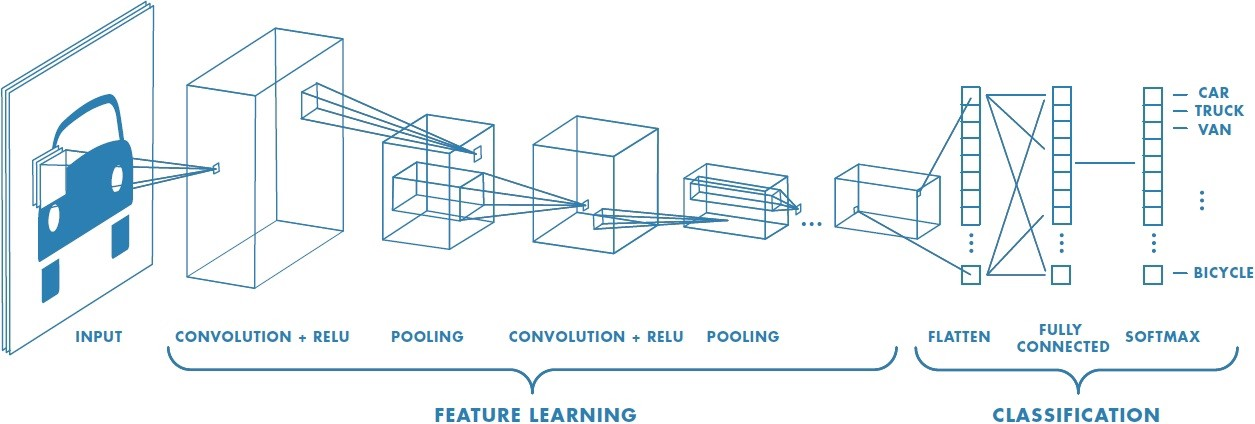
\includegraphics[width=1.0 \linewidth]{cnn.jpeg}
    \caption{Deep Convolutional Neural Networks Architecture}
\end{figure}

\paragraph{Convolutional Layer (CONV)} computes the corresponding output of neurons that are connected to a set of positions in the input matrix. 

\paragraph{Normalization Layer} also known as the Rectifier Layer (RELU) works as a filter by applying a threshold that would keep the volume of the image unchanged but implicitly performing an element-wise activation function to format the result statistically as a value ranging between ${0 \rightarrow 1}$. 

\paragraph{Pooling Layer (POOL)} reduces the complexity of image by downgrading the spatial dimensions, specifically height and width.

\paragraph{Fully Connected Layer (FC)} classifies the given object against a set of predetermined classes by estimating the accuracy scores for each class, then choosing the one with the highest probability.



\subsection{Color Thresholding \& Edge Detection} Additionally, We used a combination of color and gradient thresholds along with an edge detection algorithm to create a bitmap of zeros and ones that locates the exact pixels of the road markers. 

\paragraph{Camera Calibration and Frame Undistortion: } 3D objects are normally transformed into 2D projections of the objects in a 2D-space, which causes various levels of distortion depending on the camera used to take the picture. We start by preparing (object points), which will be the (x, y, z) coordinates of the chessboard corners in the original image. We then used the output \textit{object\_points} and \textit{image\_points} to compute the camera calibration and distortion coefficients using the \textbf{cv2.calibrateCamera()} function. We applied this distortion correction to the test image chessboards using the \textbf{cv2.undistort()} function and obtained this result:

\begin{figure}[!h]
	\centering
    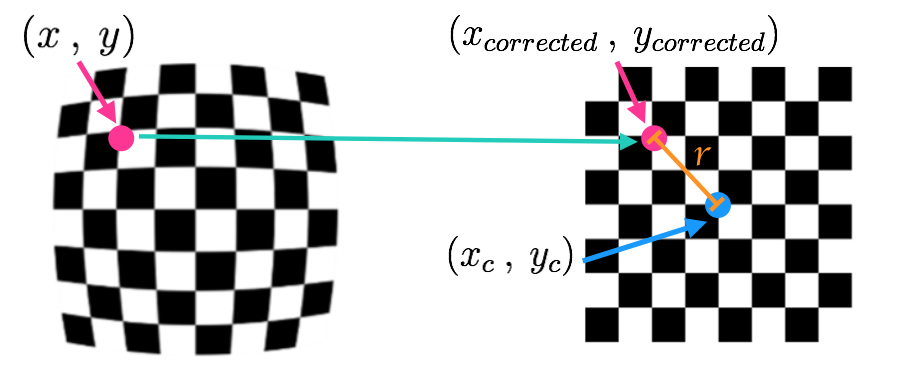
\includegraphics[width=1.0 \linewidth]{lane-undistortion.png}
    \caption{Camera Calibration and Frame Undistortion}
\end{figure}

\paragraph{HSV Mask: } First, we applied an HSV mask to the undistorted image, which helps to extract the yellow lines by focusing on the hue and saturation of the pixel and not so much on how dark the pixel might be.


\paragraph{Canny Edge Detection: } It is a technique widely used in computer vision systems to essentially extract structural information from an image and dramatically reduce the amount of data that needs to be be processed. We applied this operator only to the bottom half of the image assuming that our region of interest is only the lower section of the input image where lane markings are expected to be.

\pagebreak

\paragraph{Gaussian Noise: } Then, we take the resulting image from our edge detection algorithm and apply \textbf{cv2.equalizeHist}, followed by \textbf{cv2.GaussianBlur}, which improves the contrast of the image to easily detect any white road marks and remove any noise in the image. 

\begin{figure}[h!]
  \centering
  \subfigure[HSV Mask]
  {%
    \label{fig:first}%
    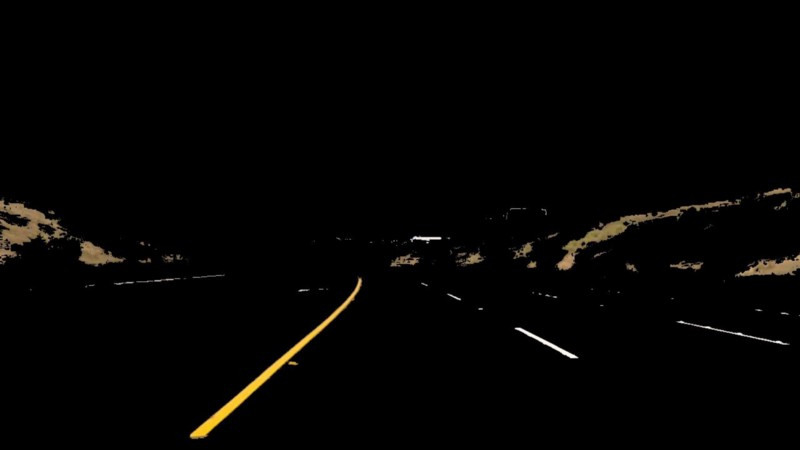
\includegraphics[width=.45 \linewidth]{lane-hsv.jpeg}
  }%
  \qquad
  \subfigure[Canny Edge Detection]
  {%
    \label{fig:second}%
    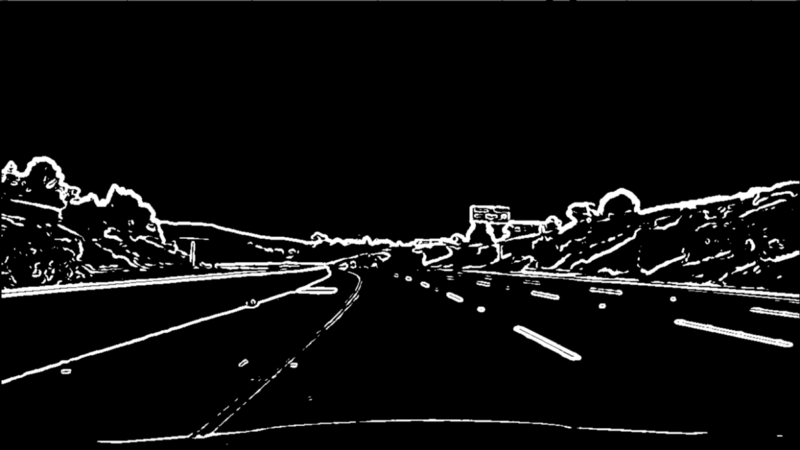
\includegraphics[width=.45 \linewidth]{lane-canny.png}
  }%
  \qquad
  \subfigure[After Removing Gaussian Noise]
  {%
    \label{fig:third}%
    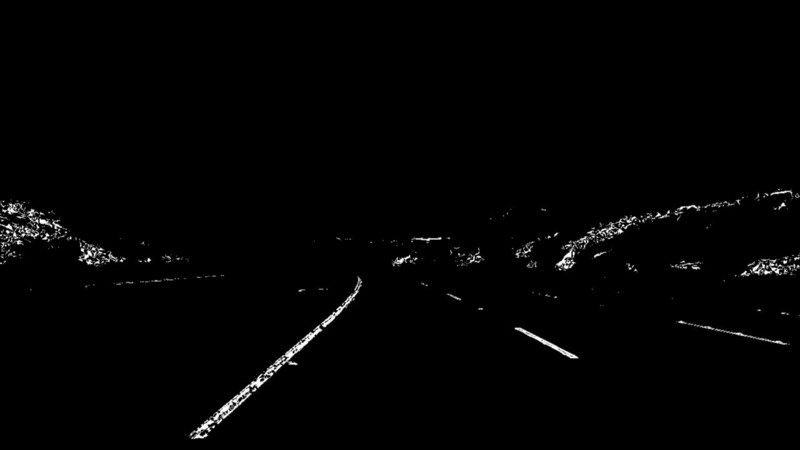
\includegraphics[width=.75 \linewidth]{lane-gaussian.jpeg}
  }%
  \caption{Color Thresholding \& Edge Detection}
\end{figure}


\paragraph{Perspective Transform: } This is a very basic, yet crucial step to figure out the lane curvature. The idea is to map the pixels in a given image to a bird's-eye view, in order to view a lane from above.  This requires \textbf{cv2.getPerspectiveTransform} and \textbf{cv.warpPerspective}.


\paragraph{Sliding Window Search: } For this step, we apply an intensive search to identify the exact pixels corresponding to the road marks. Starting from the very bottom of the image, we insert two windows, one for each peak point of the histogram of the bitmap. We then adjust the window's position based on the average density of pixels within the given window and slide the windows upwards until we reach the end of the image. Lastly, we draw a line through the center points of the windows to represent the lane boundary.

\begin{figure}[h!]
  \centering
  \subfigure[Bird's-eye view (bitmap)]
  {%
    \label{fig:first}%
    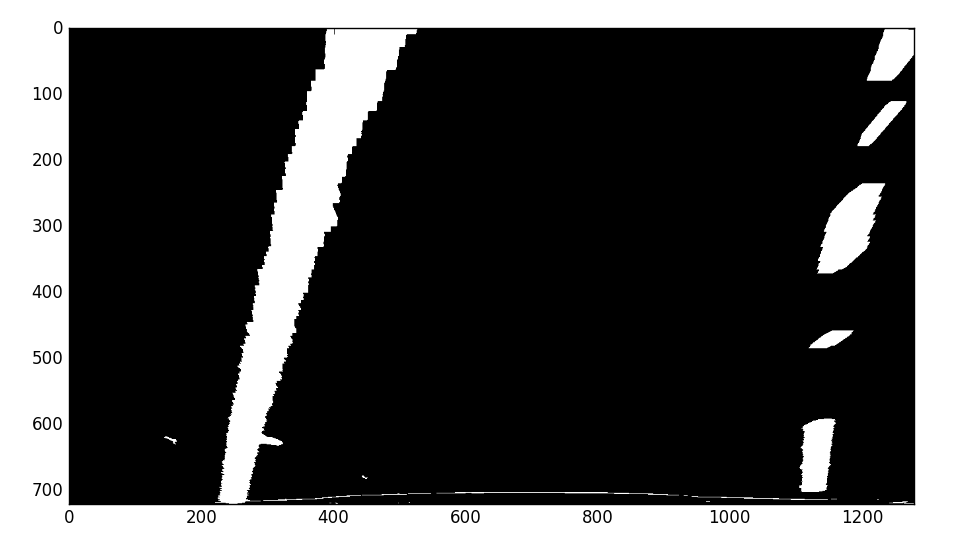
\includegraphics[width=.45 \linewidth]{lane-bitmap.png}
  }%
  \qquad
  \subfigure[Bitmap Histogram]
  {%
    \label{fig:second}%
    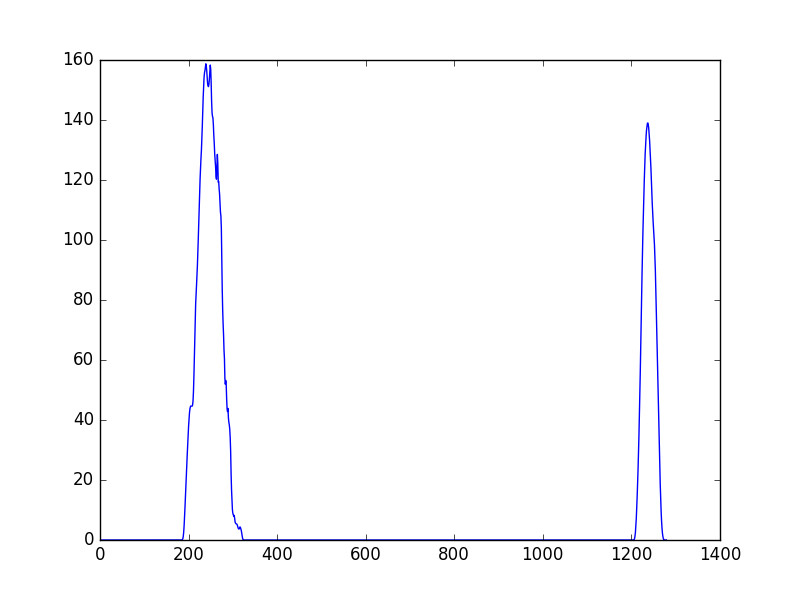
\includegraphics[width=.45 \linewidth]{lane-histogram.png}
  }%
  \qquad
  \subfigure[Bird's-eye view (lane detected)]
  {%
    \label{fig:third}%
    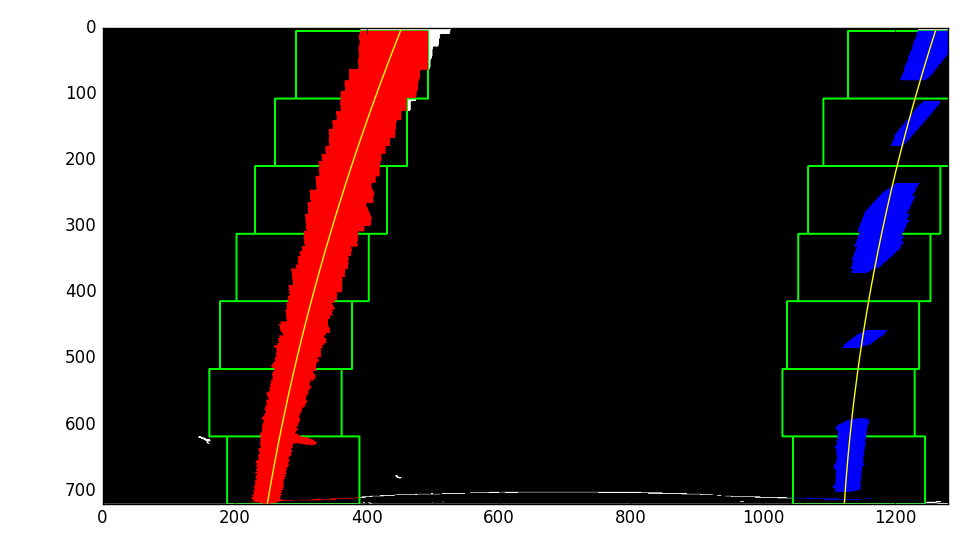
\includegraphics[width=.75 \linewidth]{lane-detected.png}
  }%
  \caption{Sliding Window Search}
\end{figure}

\pagebreak

\paragraph{Sliding Window Search Optimization: } Initially, the lane detector was hard-coded to detect lane-pixels by focusing on the bottom-half of the frame. Then, we updated our \textit{LaneDetector} class to adopt various frame sizes. It now captures one-third of the frame vertically, and two-thirds of the frame horizontally starting from the center (illustrated in the graph below). 

\begin{figure}[h!]
	\centering
    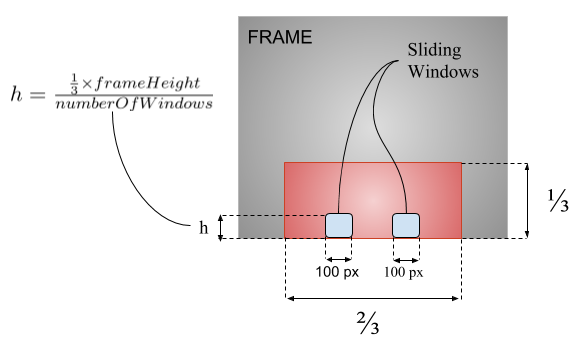
\includegraphics[width=.75 \linewidth]{lane-sliding-windows.png}
    \caption{Sliding Window Search Optimization}
\end{figure}

\pagebreak

\paragraph{Collision Detection} We limited pedestrian warnings to people who are crossing in front of the driver only. Furthermore, we limited vehicle and bike warnings by excluding any objects that are detected outside of a predefined area in the given frame (our main region of interest (ROI) highlighted in yellow in the graph below). This is so warnings are not given for distant objects.  In addition, we created a collision warning, which alerts the driver if there’s a potential collision with an object very close to the car. This uses an even smaller box (the collision ROI) at the bottom of a given frame, and checks if the bottom of an object was detected within the \textbf{COLLISION ROI} highlighted in red in the graph below.

\begin{figure}[h!]
	\centering
    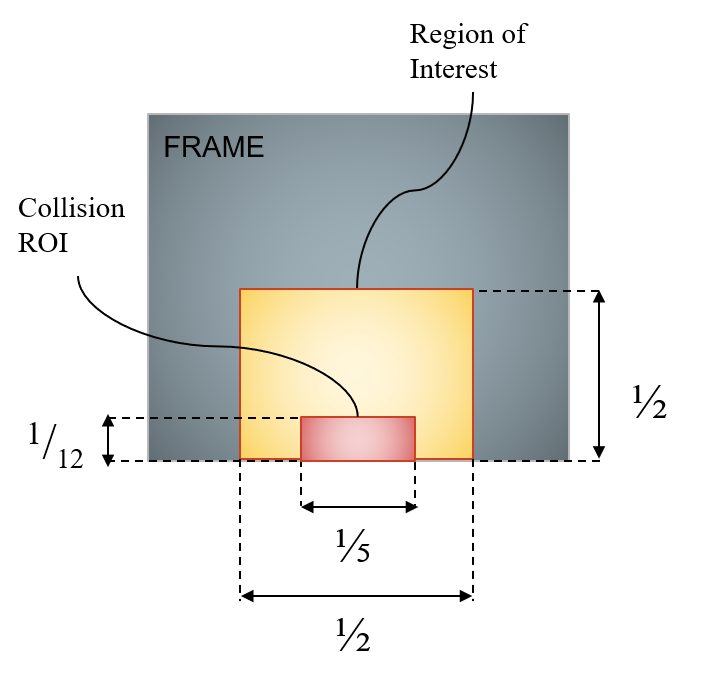
\includegraphics[width=.55 \linewidth]{roi.png}
    \caption{Detection | Region of Interest (ROI)}
\end{figure}

%-------------------------------------------%

\pagebreak

\section{Analytical Methods}
%-------------------------------------------%

\paragraph{Benchmark:} We added a diagnostic mode option that allows us to run some testing scripts to evaluate the system performance in various situations. When you run the system in diagnostic mode, the system will take 10-15 screenshots every minute (varies based on the frame rate). Each screenshot demonstrates a given frame captured by our system prior to our sense analysis and after our detection and classification. 

\begin{figure}[h!]
  \centering
  \subfigure[Pre — Scene Recognition]
  {%
    \label{fig:first}%
    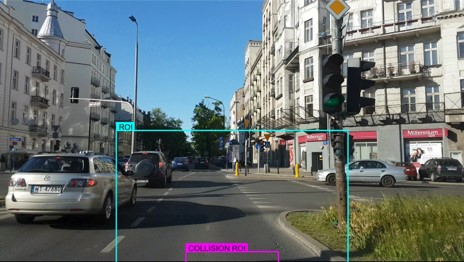
\includegraphics[width=.45 \linewidth]{pre.jpg}
  }%
  \qquad
  \subfigure[Post — Scene Recognition]
  {%
    \label{fig:second}%
    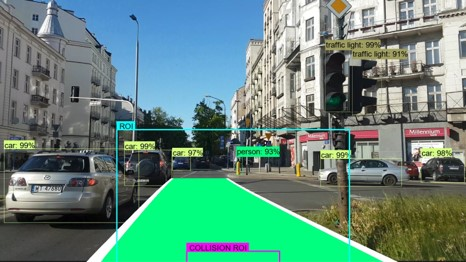
\includegraphics[width=.45 \linewidth]{post.jpg}
  }%
  \caption{Diagnostic Mode}
\end{figure}

Then, we made a \textbf{pandas} data frame that stores the ID of the captured frame along with a set of attributes that were detected in the given frame. Each screenshot will be associated with a data entry that gets generated automatically to describe the given frame, and will eventually save to a CSV file with a timestamp to indicate when it was done. Finally, each data entry in our log files will get an “accuracy” score based on the true/false positive predictions, then we will calculate an average score to express how well the system is doing.  

\begin{figure}[h!]
	\centering
    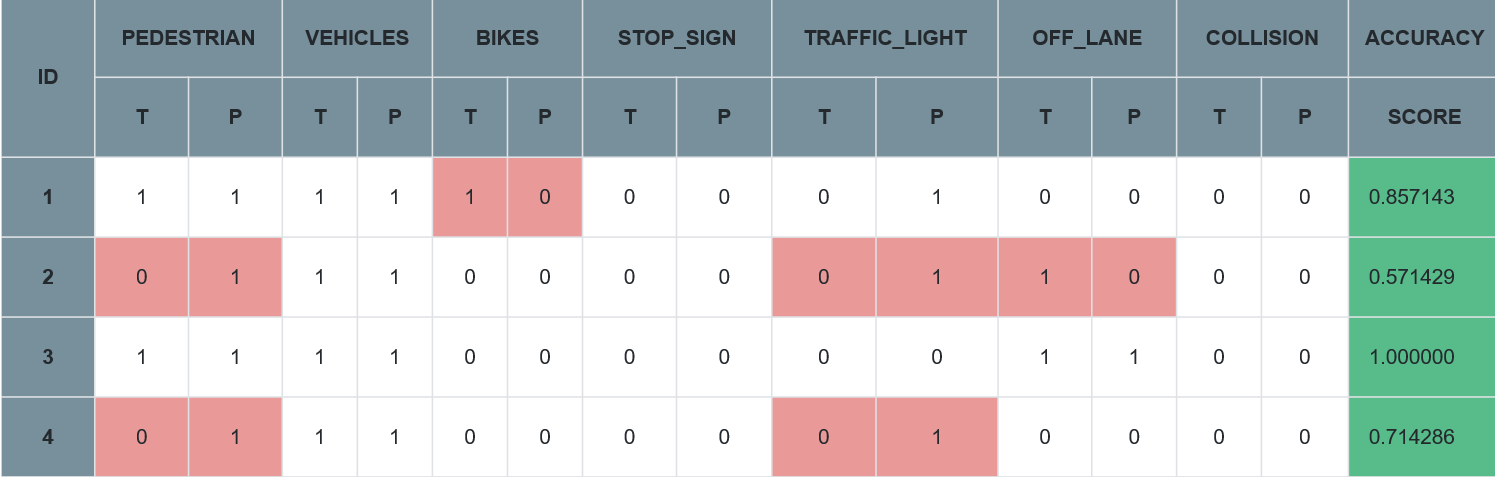
\includegraphics[width=1.0 \linewidth]{data-log.png}
    \caption{Data Log}
\end{figure}

\pagebreak

\paragraph{Practical/Visual Testing:} Additionally, we will test the program ourselves and compare the output with what we would have estimated if we were driving the car.

\paragraph{Hands-On Experience:} Lastly, we evaluated our system in the settings of Grand Theft Auto V, as it was gratifying to watch the system in-action with somebody driving a vehicle in the game with DeepEye operating behind the scenes as a copilot assisting the driver. Being a virtual environment, this also allowed us to easily test in many different driving environments, weather conditions, and times of day. 

%-------------------------------------------%


\section{Features}
%-------------------------------------------%
\paragraph{Object/Lane Detection \& Scene Recognition:} This will be our most fundamental feature, which is required for all else to function.  TensorFlow and OpenCV will be used to do this, using a Convolutional Neural Network.  This system will create tight bounding boxes around objects, and classify them as other vehicles, pedestrians, bicycles, lanes, street signs, etc.
\par

\paragraph{Copilot -- Advanced Driver-Assistance System (ADAS):} This feature determines if the objects detected pose a potential threat to the driver. To do this, it takes the type of object and its trajectory into account.  Context is important; oncoming traffic in the other lane will get close to the driver, but does not normally pose a threat. In this case, trajectory is most important. As long as the other car does not intersect with the driver's trajectory, there is no threat posed.  If an potential collision is detected, an audible warning will alert the driver. The following is a list of warnings given:

\begin{itemize}
\item Pedestrians nearby
\item Vehicles nearby
\item Bikes/Motorcycles nearby
\item Stop sign ahead
\item Traffic light ahead
\item Forward collision warning
\item Lane departure warning
\end{itemize}

%-------------------------------------------%

\pagebreak

\section{Test Plan}
%-------------------------------------------%

An important part of the project will be analyzing the accuracy of our scene recognition. The system would be easily tested on videos that are publicly available online (collected from a camera mounted on the front windshield of a vehicle). Our plan is to test our system on a set of videos; we will then provide some statistical charts for the accuracy of our object/lane detectors. Once the system passes the object detection test, we will evaluate the system's performance ourselves visually by comparing the output of the warning interface to what would be expected if we were in the same situation. Through extensive visual testing, we would be able to highlight any unnecessary warnings and/or outliers in the system. At the final testing stage, we demonstrated our system in Grand Theft Auto V, which allowed us to control the environment surrounding our agent, and test our system on various weather/lighting conditions.

%-------------------------------------------%


\section{Criteria and Constraints}
%-------------------------------------------%

The biggest constraint is our limited access to powerful hardware resources. Notably, most machine learning applications, particularly the ones that rely on computer vision, require advanced and super optimized GPUs to process the frames that are imported into the system accurately and efficiently. Unfortunately, we only had a single Titan Xp, while a real-time ADAS would probably use a set of Tesla/Quadro GPUs, which are more powerful and highly optimized for deep-learning and computer-vision tasks.

%-------------------------------------------%